\documentclass[11pt,letterpaper,fleqn]{article}

% Load packages
\usepackage{fancyhdr}
\usepackage{graphicx}

% --- SETUP PAGE HEADER --- %
\pagenumbering{arabic}
\pagestyle{fancy}
\fancyhf{}
\fancyhead[L]{\textsl{The Ising Model}}

% You should only need to change the following line in this section
\fancyhead[R]{\textsl Page \thepage}


%%%%%%%%%%%%%%%%%%%%%%%%%%%%%%%%%%%%%%%%%%%%%%%%%%%%%%%%%%%
%%%%%%%%%%%%%%%%%%%%%BEGIN DOCUMENT%%%%%%%%%%%%%%%%%%%%%%%%
%%%%%%%%%%%%%%%%%%%%%%%%%%%%%%%%%%%%%%%%%%%%%%%%%%%%%%%%%%%
\begin{document}

% <--- TITLE START ---> %
\begin{center}
{\Large \textbf{Phase Transitions and the Ising Model}}\\
{International Course on Computational Physics}\\
{Michigan State University and Delft University of Technology}\\
\vspace{0.15in}
{Jared Doster and Chiel Donkers}\\
{April 5, 2013}\\
\end{center}
% <---- TITLE END ----> %


%%%%%%%%%%%%%%%%%%%%%%%%%%%%%%%%%%%%%%%%%%%%%%%%%%%%%%%%%%%
\section*{Introduction}

The purpose of this paper is to report on the results of multiple simulations pertaining to phase transitions in 
two-dimensional spin lattices.  All lattices studied were square and contained only spin $frac{1}{2}$ particles.
The simulations investigated...

The simulations were coded in FORTRAN90.


We will first discuss the physics of the Ising model.  Then, we will discuss the multiple algorithms used to study then
Ising model.  Finally, we will investigate specific results of the simulations.
\newline


%%%%%%%%%%%%%%%%%%%%%%%%%%%%%%%%%%%%%%%%%%%%%%%%%%%%%%%%%%%
\section*{The Ising Model}

The purpose of the Ising model is to describe the dynamics of phase transitions in ferromagnetic materials.  The one-dimensional
Ising model, which has no phase transitions, was solved by Ernst Ising in 1925.  The two-dimensional sqare lattice Ising model 
was analytically studied Lars Onsager in 1944.  


In the Ising model, The Hamiltonian of a spin $\frac{1}{2}$ ferromagnet of a general shape is
\[
H = -J \Sigma_{ij} S_{i} S_{j}
\]
where $J>0$ is a ferromagnetic exchange constant, $S_{i} = \pm1$ is a spin variable, and the summation is over the nearest-neighbor
sites on the lattice.

The quantity that characteristically describes any magnet is the magnetization $m$, which is defined as
\[
m = \frac{\Sigma_{i} <S_{i}>}{N}
\]
where $N$ is the total number of spin particles in the ferromagnet.  


The properties of all magnetic materials change as a function of the temperature of the material.  A quantity of interest is the
Curie temperature $T_{c}$, which is defined as the temperature at which a magnetic material looses its permanent magnetism.  
In other words, at $T_{c}$ am ``order-to-disorder'' phase transition occurs in the orientations of the spins of the ferromagnet. 
At temperatures higer than $T_{c}$, the magnet is very susceptible to induced magnetization.
\newline


%%%%%%%%%%%%%%%%%%%%%%%%%%%%%%%%%%%%%%%%%%%%%%%%%%%%%%%%%%%
\section*{Monte Carlo Methods}

The analytical description of the Ising model is impractical to use because transitions near $T_{c}$ exhibit complex phenomena.
In light of this, the Ising model has been extensively studied by use of Monte Carlo methods.


Monte Carlo methods were first studied during the Manhatten project in the 1940s and serve to deepen our theoretical understanding
of physical phenomena.



%%%%%%%%%%%%%%%%%%%%%%%%%%%%%%%%%%%%%%%%%%%%%%%%%%%%%%%%%%%
\subsection*{Metropolis Algorithm}

The Metopolis Algorithm was first published in 1953 and is considered to by the most widely used Monte Carlo algorithm.
Simply put, it is a method for obtaining a sequence of random values from a probability distribution. This sequence can be used
in numerous applications such as approximation of multi-dimensional distributions, numerical integration, and graph theory. 

The outline of the mainloop of Metropolis algorithm, as applied to the Ising model, is as follows:
\newline

(i) Randomly choose a location in the lattice randomly.
\newline

(ii) Calculate the energy difference $\delta E$ between the spin up and spin down orientations.
\newline

(iii) Calculate the expression $e^{\beta \delta E}$
\newline

(iv) Let $x$ be a random number on the internal $[0,1]$.  If $e^{\beta * \delta E} > x$, then flip 
the randomly selected spin.
\newline

(v) Calculate the magnetization by averaging over the orientation of all spins.
\newline

(vi) If satisfied with the value for the magnetization, exit the loop.  If not satisfied, return to (i).
\newline


The above loop iterates over arbitrary time steps.  After some time, the value for the magnetization should converge to a ``small'' 
range of values.  The size of this ``smallness'' is determined by the needs of the experimenter.


%%%%%%%%%%%%%%%%%%%%%%%%%%%%%%%%%%%%%%%%%%%%%%%%%%%%%%%%%%%
\subsection*{Cluster Algorithms}


In the above Metropolis algorithm, one randomly selected spin is updated (flipped or not flipped) for each sweep across the 
entire spin lattice, which is computationally expensive. Also, at temperatures near the critical temperature, there is a large
increase in fluctuations in total magnetization and total energy, which requres more measurements to reduce the statistical noise.


In the late 1980s, research began on new algorithms that would reduce the two issues stated in the previous paragraph.
This would be achieved by updating clusters of spins for each sweep across the lattice.  
In these methods, the difficulty is in creating a method that effeciently and effectively
identifies the appropriate clusters to be updated.  In the case of the Ising model, the clusters are continuous groups
of particles with the same spin orientation.


%%%%%%%%%%%%%%%%%%%%%%%%%%%%%%%%%%%%%%%%%%%%%%%%%%%%%%%%%%%
\subsubsection*{Wolff Algorithm}

In the Wolff algorithm, a single cluster is updated for each sweep of the lattice.


The outline of the algorithm as it is applied to the Ising model is as follows:
\newline

(i) Randomly choose a location in the lattice randomly.
\newline

(ii) There are eight nearest-neighbor locations to the randomly selected location.  Choose a nearest-neighbor location
of the same orientation as the spin in the first selected location.  The choice does not have to be random.
\newline

(iii) Let $x$ be a random number on the internal $[0,1]$. If $1 - e^{\frac{2J}{u_{\beta}T}} > x$, then add the 
nearest-neighbor spin to the cluster.
\newline

(iv) After growing the cluster to completion, flip the cluster.
\newline

(v) Continue 
\newline


%%%%%%%%%%%%%%%%%%%%%%%%%%%%%%%%%%%%%%%%%%%%%%%%%%%%%%%%%%%
\subsubsection*{Swendsen-Wang Algorithm}

Unlike the Wolff algorith, the Swendsen-Wang algorithm updates multiple clusters for each sweep of the lattice.




%%%%%%%%%%%%%%%%%%%%%%%%%%%%%%%%%%%%%%%%%%%%%%%%%%%%%%%%%%%
\section*{Simulations and Results}

We ran simulations of the ising model for all three algorithms: Metropolis, Wolff, and Swendsen-Wang.
The purpose of these simulations is to investigate the Magnetization as a function of both time and temperature
for different computational algorithms.


%%%%%%%%%%%%%%%%%%%%%%%%%%%%%%%%%%%%%%%%%%%%%%%%%%%%%%%%%%%
\subsubsection*{Metropolis Algorithm}

The following plot is magnetization versus time.  For this plot, we chose a temperature of 2.5.  
Note that the critical temperature for phase transition is 2.3.

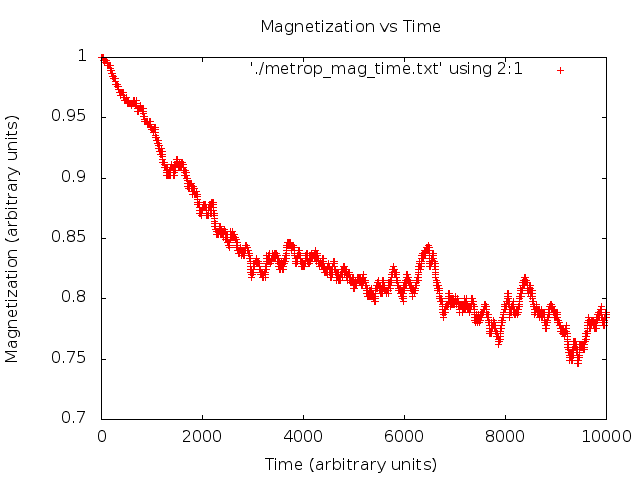
\includegraphics[width=1\textwidth]{images/metrop_mag_time.png}


The following plot is magnetization versus temperature. As one can see, our simulation does not properly replicate
the critical temperature of 2.5.  The magnetization begins to substantially drop toward zero around 2.5.

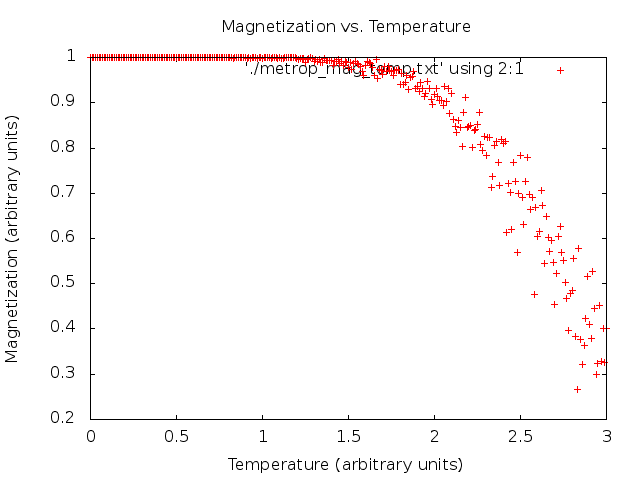
\includegraphics[width=1\textwidth]{images/metrop_mag_temp.png}



%%%%%%%%%%%%%%%%%%%%%%%%%%%%%%%%%%%%%%%%%%%%%%%%%%%%%%%%%%%
\subsubsection*{Cluster Algorithms}

The following plot is for the Swendsen-Wang Algorithm.

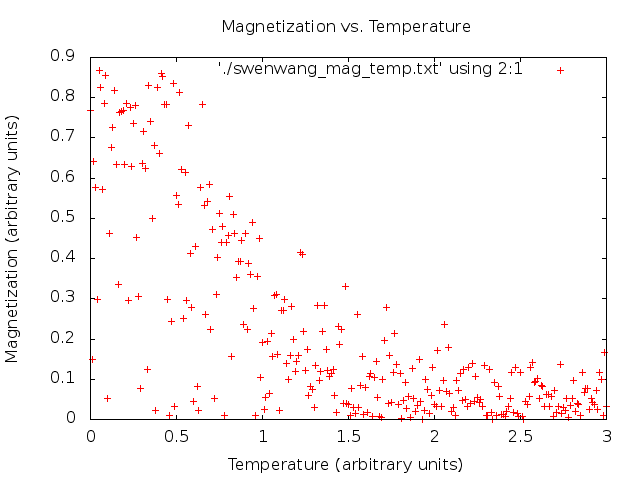
\includegraphics[width=1\textwidth]{images/swenwang_mag_temp.png}




%%%%%%%%%%%%%%%%%%%%%%%%%%%%%%%%%%%%%%%%%%%%%%%%%%%%%%%%%%%
\subsubsection*{Wolff Algorithm}

The following plot is for the Wolff Algorithm.

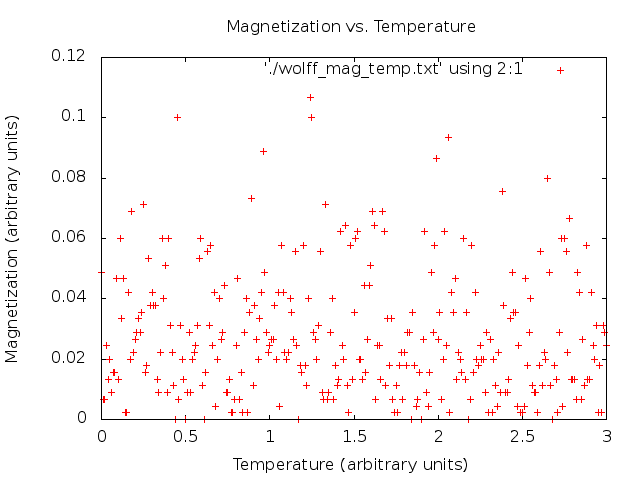
\includegraphics[width=1\textwidth]{images/wolff_mag_temp.png}









\end{document}